% Emacs, this is -*-latex-*-
\documentclass[12pt]{ugentreport}
\usepackage[a4paper]{geometry}
\geometry{a4paper,margin=3cm,marginparwidth=20mm}
\usepackage[dutch]{babel}
\usepackage{parskip}
\usepackage{amsfonts}
\usepackage{amsmath}
\usepackage{cancel}
\usepackage{commath}
\usepackage{amssymb}
\usepackage{parskip}
\usepackage{rotating}
\usepackage{listings}
\usepackage{siunitx}
\usepackage{graphicx}
\usepackage{geometry}
\usepackage{underscore}
\usepackage{tikz}
\usepackage[dutch]{todonotes}
% Gives me \intertext and \shortintertext
\usepackage{mathtools}
\usepackage[european, siunitx]{circuitikz}
\usetikzlibrary{calc}
% Nicer unit fractions
\sisetup{per-mode=fraction}
% Smaller margins
% \usepackage{fullpage}
% Clickable links
\usepackage{hyperref}

\lstMakeShortInline[basicstyle=\ttfamily,language=C]{§}

\title{Verslag Project Microcontrollers}
\author{Marieke Louage\and Stef Pletinck}

\begin{document}

\maketitle

\tableofcontents
\listoffigures
\newpage

\section{Doelstellingen}
Doel van deze opgave was het maken van een spel op een microcontroller,
specifiek een \emph{AT90USB646} op een \emph{Dwenguino} ontwikkelbord.
Verdere doelen van het vak zijn het leren lezen en interpreteren van datasheets
en werken met de taal \emph{C}.
Er werd besloten om een multiplayer spel te maken,
voor meer interactiviteit.

Voor de weergave van het spel werden verschillende mogelijkheden overlopen.
Een eerste mogelijkheid was het aansturen van een VGA-display,
maar door de hoge klokfrequentie van VGA en de daaraan gelinkte problemen
werd dit idee snel verworpen.
Een tweede idee was het gebruik van een LED-matrix.
De lage resolutie hiervan was echter een groot nadeel,
dus werd uiteindelijk gekozen voor een scherm dat gebruik maakt
van het principe van een hardeschijfklok. Een snel ronddraaiende ledstrip werd
ook overwogen, maar dit is praktisch niet haalbaar.

Het spel zelf vindt plaats in een baan rond de aarde, waar twee ruimteschepen
elkaar rond de aarde achtervolgen en proberen neer te schieten.

Als invoer van de spelers werd gekozen voor arcade-joysticks.
Deze bestaan uit vier microswitches per joystick.
Er waren verder nog vele ideeën om het spel verder uit te breiden.

\section{Praktische aanpak}
De nodige functionaliteit werd opgedeeld in logische blokken die met elkaar
communiceren en op elkaar vertrouwen voor informatie. De bekomen structuur is
zichtbaar in figuur~\ref{fig:structuur}.
Op deze figuur staat hardware in ovalen en software in rechthoeken.

Het motorsysteem staat los van alles, en genereert op basis van interrupts het
controlesignaal voor de hardwarematige motordriver, die de hardeschijfmotor
aanstuurt.

Een optische sensor genereert interrupts die worden geïnterpreteerd tot
timinginformatie over de draaischijf. Deze worden gebruikt door het
\emph{graphics} systeem om de juiste LED's te laten oplichten. Dit systeem wordt
constant vanuit een lus in §main()§ opgeroepen, en geeft door welke LED's moeten
oplichten aan de \emph{leddriver}, die de feitelijke seriële data genereert en
blokkerend doorstuurt naar de LED's.

De gegevens voor het \emph{graphics} systeem worden gegenereerd door de
\emph{engine}, die via een interrupt 30 keer per seconde alle objecten in het
spel ververst en doorgeeft aan \emph{graphics}. Daarvoor worden gegevens over de
joysticks synchroon uitgelezen door het \emph{joysticks} systeem.

\begin{figure}
  \centering
  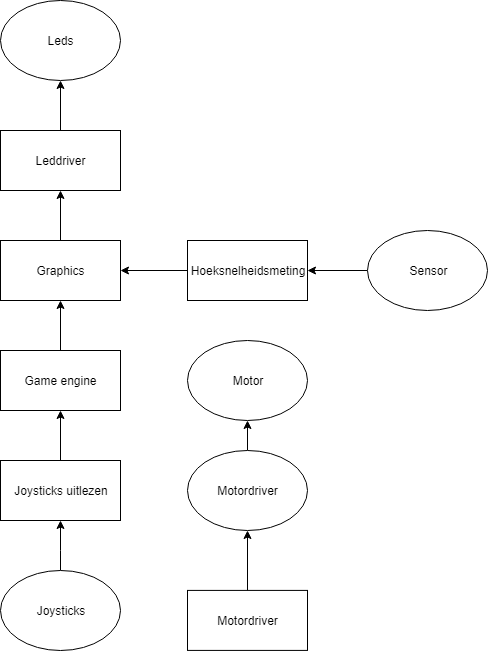
\includegraphics[width=0.8\textwidth]{img/structuur.png}
  \caption{Structuur van het microcontrollerprogramma}
  \label{fig:structuur}
\end{figure}


\subsection{Werking display}
Een schijf met gaten draait snel rond over LED's, verspreid in sectoren, zie figuur~\ref{fig:schijf}
Door de LED's op de gepaste momenten in en uit te schakelen
kan een zeer hoge resolutie bekomen worden rond het middelpunt.
In de radiale richting is de resolutie beperkt door het aantal LED's,
dit werd oorspronkelijk gekozen op 16 om de aansturing werkbaar te houden.
Er bleek dat er, door de dunne wanden tussen sectoren, soms twee ``pixels''
zich boven dezelfde sector bevonden en \emph{spookpixels} weergaven,
dus is het aantal sectoren behouden op 16,
maar werd besloten om in de radiale richting naar 13 pixels te gaan.

Met deze aanpak is het mogelijk om willekeurig de resolutie te kiezen
waarmee de hoek wordt beschreven. Hoe groter deze resolutie,
hoe meer pixels. Deze waarde werd gekozen op \num{3600}, dit als een goede balans
tussen nauwkeurigheid van het display en haalbaarheid. Hoe hoger deze resolutie,
hoe sneller de LED's namelijk ververst moeten worden om te zorgen dat alle
objecten weergegeven worden. Deze limietwaarde maakt het ook makkelijk om hoeken
in graden om te rekenen naar hun interne waarde.

\begin{figure}
  \centering
  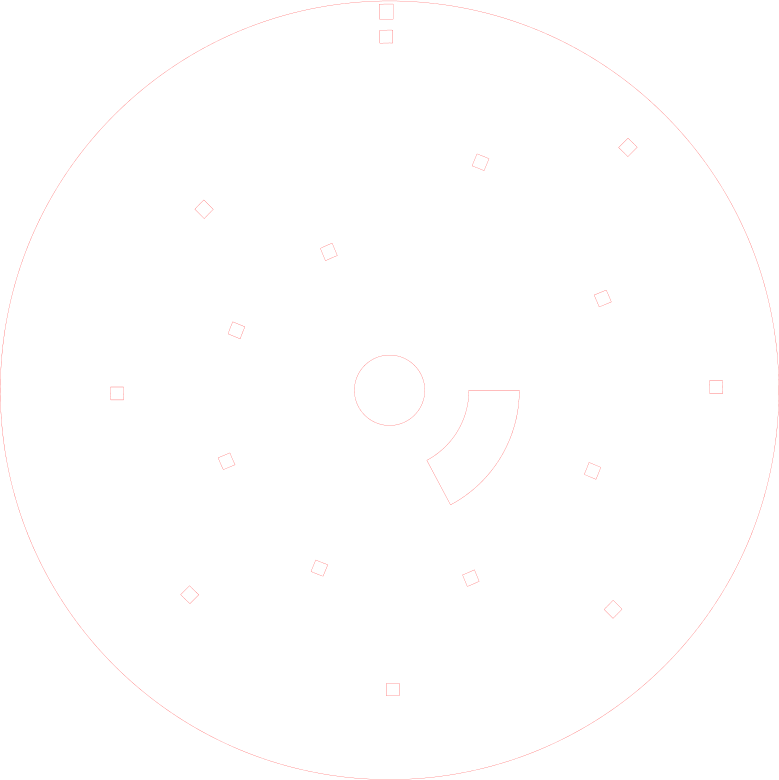
\includegraphics[width=0.6\textwidth]{img/schijf.jpg}
  \caption{Schema van de draaischijf}
  \label{fig:schijf}
\end{figure}

\subsection{Aansturing motor}
De schijf draait rond met behulp van een brushless DC-motor uit een harde schijf.
Om deze aan te sturen is een speciale ESC-module\footnote{ESC: Electronic Speed Control} nodig.

Deze modules zijn ontworpen voor gebruik in quadcopters en verwachten bijgevolg
een speciale aansturing.
Het nodige signaal is een vorm van PWM, met een frequentie van 50 of
\SI{60}{\hertz}
en een pulsbreedte tussen $1$ en \SI{2}{\milli\second}.
De PWM-modules die ingebouwd zitten in de microcontroller kunnen niet opereren
in deze frequenties en pulsbreedtelimieten,
het protocol werd dus volledig in software geïmplementeerd.
Zie figuur~\ref{fig:motorpwm} voor een beeld van het geproduceerde signaal.

Het PWM signaal wordt op pin §D0§ naar buiten gebracht. De software implementatie
van het PWM signaal is met Timer/Counter3 in Clear Timer on Compare Match (CTC)
modus verwezenlijkt. In het register OCR3A wordt een waarde ingesteld, wanneer de Timer/Counter
deze waarde bereikt wordt de counter op nul gezet en wordt de interrupt §TIMER3_COMPA_vect§
aangevraagd. Er wordt in de interrupt service routine een nieuwe waarde ingesteld
in §OCR3A§ en de output bit op pin §D0§ wordt geflipt. Deze counter werd gekozen
vanwege zijn 16-bits resolutie.

Om nul procent vermogen aan te sturen moet het signaal \SI{1}{\milli\second} hoog zijn, om het
maximale vermogen aan te sturen moet het signaal \SI{2}{\milli\second} hoog zijn. De Timer/Counter3
heeft een frequentie van \SI{2}{\mega\hertz}, dat is de \texttt{I/O} klok van \SI{16}{\mega\hertz} verschaald met
prescaler $8$. Een voorbeeld van het PWM signaal dat overeenkomt met \SI{0}{\percent}
motorvermogen is in tabel~\ref{tbl:PWM} zichtbaar.

\begin{table}
  \centering
  \begin{tabular}{rSS}
    \hline
    & {Klokslagen} & {Tijd (\si{\milli\second})}\\
    \hline
    Hoge puls & 2000 & 1\\
    Lage puls & 38000 & 19\\
    \hline
    Periode & 40000 & 20\\
    \hline
  \end{tabular}
  \caption{PWM generatie}
  \label{tbl:PWM}
\end{table}

\begin{figure}
  \centering
  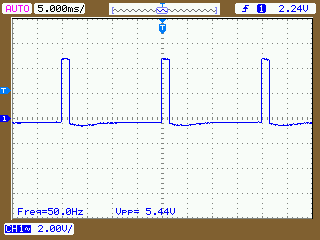
\includegraphics[width=0.6\textwidth]{img/scoopcontrolesc.png}
  \caption{Controlesignaal ESC}
  \label{fig:motorpwm}
\end{figure}

Een extra moeilijkheid is de opstartprocedure van de ESC.
De microcontroller moet opgestart zijn en een signaal sturen dat overeen komt
met \SI{0}{\percent} motorvermogen wanneer de ESC stroom krijgt en wordt
ingeschakeld. De ESC produceert dan een serie tonen, gevolgd door een langere
toon wanneer het signaal herkend wordt. Daarna kan de motor aangestuurd worden
en het vermogen verhoogd, liefst langzaam gezien het hoge gewicht van de draaischijf.
Uiteindelijk zal de ESC een driefasig signaal naar de motor sturen, zoals
zichtbaar in figuur~\ref{fig:motoresc}.

\begin{figure}
  \centering
  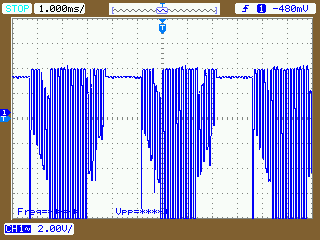
\includegraphics[width=0.6\textwidth]{img/scoopesc.png}
  \caption{Spanning naar de motor}
  \label{fig:motoresc}
\end{figure}

Deze procedure maakt het moeilijk om microcontroller en ESC op één voeding te
laten werken. Door de grote stroom is het ook lastig om bijvoorbeeld de ESC te
schakelen met een transistor. Voorlopig moet de ESC manueel in de stekker
gestoken worden. De driver wacht daartoe even met het opstarten van de motor,
aangezien de stekker pas mag ingeplugd worden wanneer het stuursignaal reeds
aanwezig is.

\subsection{Toerenteller schijf}
De hoeksnelheidsmeting component uit figuur~\ref{fig:structuur} levert de hoeksnelheid en een
ijkpunt van de draaibeweging van de schijf. Als input krijgt de component een
puls van een stationaire optische sensor die gemonteerd is langs de rand van de
schijf. In de schijf zit een gaatje waardoor de optische sensor getriggerd wordt
wanneer dit gaatje doorheen de sensor passeert. (Figuur~\ref{fig:sensor})

\begin{figure}
  \centering
  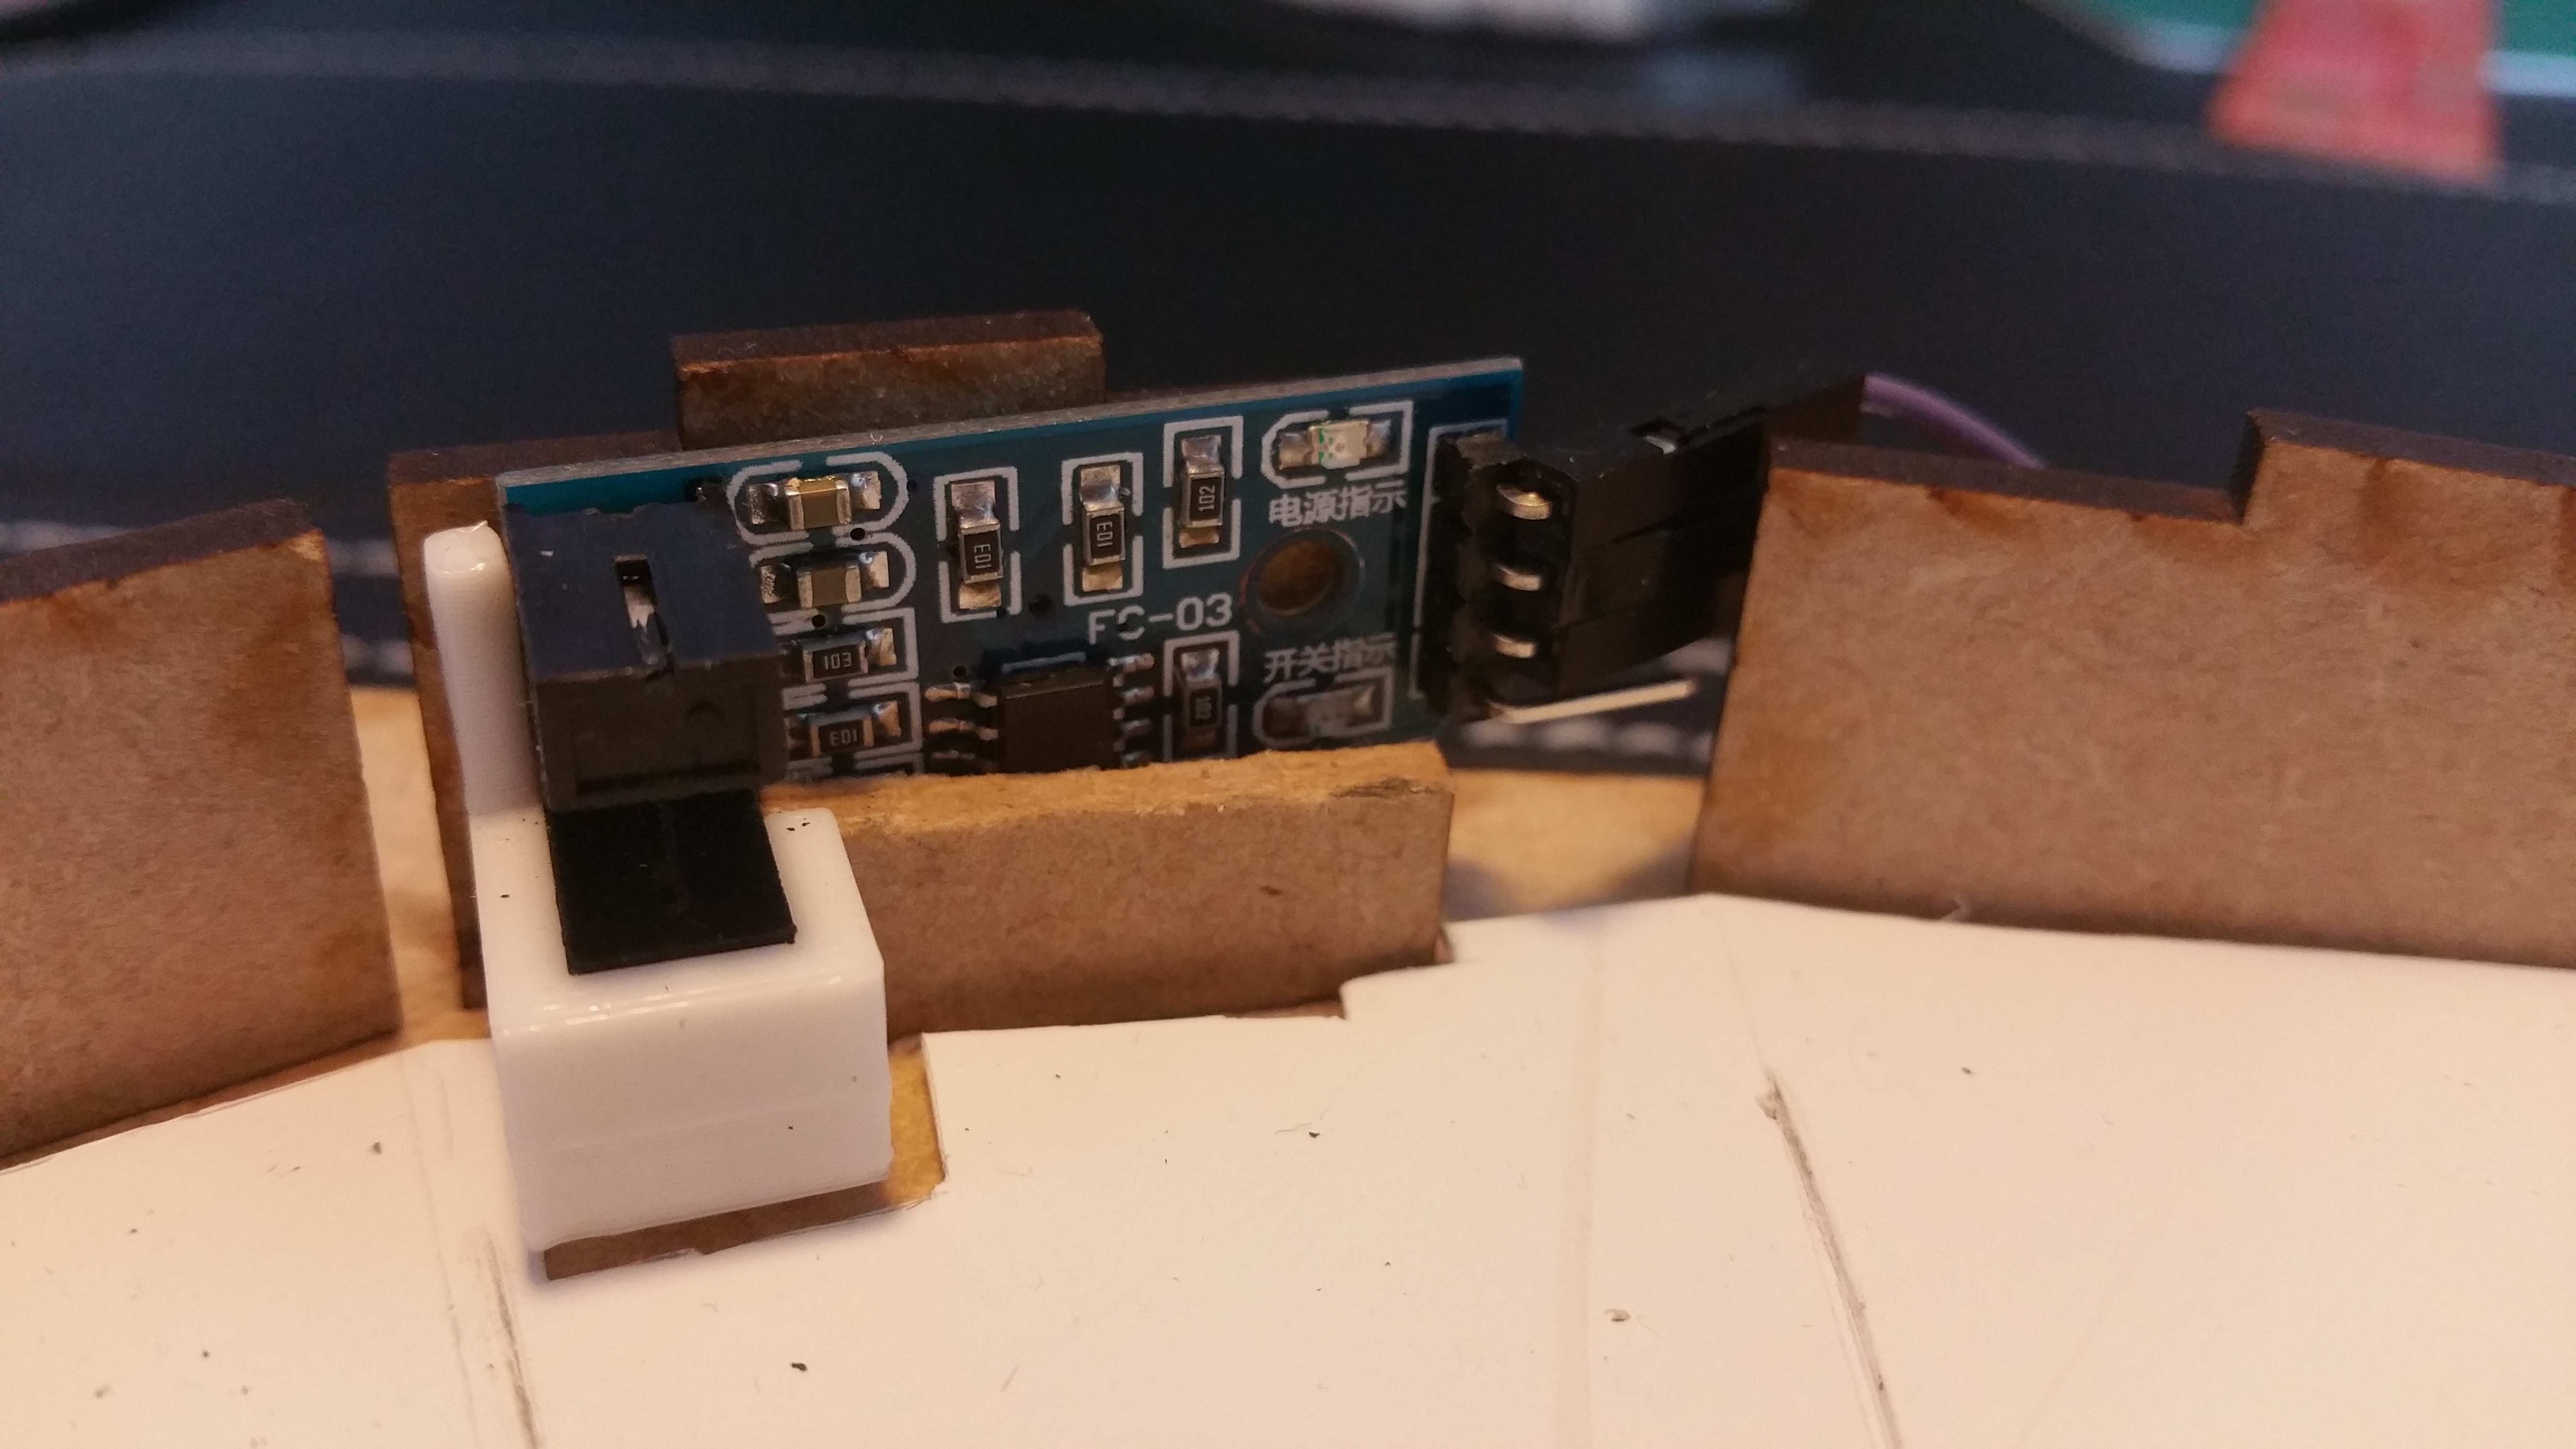
\includegraphics[width=0.6\textwidth]{img/Sensor.jpg}
  \caption{Sensor gemonteerd aan de rand van de schijf}
  \label{fig:sensor}
\end{figure}

De praktische realisatie berust op de Input Capture Unit van Timer/Counter1.
Dit vereist de alternate function van poort §PD4§, namelijk §ICP1§ of Timer/Counter1
Input Capture Trigger. Als een dalende of stijgende flank (dit is vrij te kiezen)
geregistreerd wordt op pin §ICP1§ dan wordt de huidige waarde van Timer/Counter1
zo snel mogelijk gekopieerd in een register genaamd §ICR1§, waarna dat op zijn beurt
kan bevraagd worden door de microcontroller. Doordat een noise-canceling optie aanstaat duurt
het kopiëren vier systeemklokpulsen langer, wat geen probleem levert voor de
accuraatheid.

De frequentie waarop Timer/Counter1 telt is \SI{250}{\kilo\hertz}. Dit is de \texttt{I/O} klok van \SI{16}{\mega\hertz}
verschaald met prescaler 64.

De Input Capture unit heeft de mogelijkheid tot het genereren van een interrupt.
Indien ingesteld, wordt zodra de waarde in §ICR1§ gekopieerd is, de interrupt
aangevraagd. In de interrupt routine wordt eerst de opgevangen waarde gekopieerd
om overschrijven te voorkomen
en vervolgens wordt met deze waarde de tijd die verstreken is sinds de vorige interrupt
bepaald. De eenheid van deze waarde is nog arbitrair om de hoge resolutie te bewaren,
het is een verschaalde versie van het aantal increments.

De Timer/Counter1 overflow interrupt wordt getriggerd wanneer de maximale waarde
bereikt is en de telwaarde op nul wordt gezet. Elke keer dat de overflow vector
getriggerd wordt moet het aantal increments met $216$ verhoogd worden.

In tabel~\ref{tbl:toerental} is een meting van het aantal increments te zien. Voor een hoeksnelheid van 19 toeren per seconde
is het aantal increments \num{12870}. Elke \num{65536} increments vind een overflow plaats.
De verhoudingen tussen kloksnelheid en schijfsnelheid zijn dus goed gedimensioneerd.

\begin{table}
  \centering
  \begin{tabular}{SSS}
    \hline
    {Tijd per increment (\si{\micro\second})} & {Aantal increments} & {Hoeksnelheid (toeren/s)}\\
    \hline
    4 & 12870 & 19.42502\\
    \hline
  \end{tabular}
  \caption{Meting en berekening toerental}
  \label{tbl:toerental}
\end{table}


\subsection{Aansturing LED's}
De gebruikte LED's zijn ledstrips van het type \texttt{APA102}.
Deze kunnen vrij eenvoudig via SPI data ontvangen.
SPI is een eenvoudig protocol dat bestaat uit een datalijn en een kloklijn, data
wordt seriëel op de datalijn geplaatst en kan uitgelezen worden vanaf de
stijgende flank van de klok. De gebruikte microcontroller heeft
hardwareondersteuning voor SPI, daardoor moet slechts een byte in het juiste
register geplaatst worden en de hardware zal in de achtergrond de data verzonden
worden, met automatisch de juiste kloksignalen. De klokfrequentie is via een
prescaler instelbaar tot maximaal de helft van de I/O-klok. Nadat een byte is
verzonden, wordt een vlag geactiveerd en indien gewenst een interrupt aangevraagd.

De ledstrip luistert naar nieuwe commando's na een startpakket
bestaande uit 32 0-bits. Vervolgens moet,
zoals zichtbaar op figuur~\ref{fig:ledcontrol},
een pakket per LED verstuurd worden gevolgd door
nogmaals 32 bits om te zorgen dat alle data ver genoeg doorgeschoven is.
De waarde van deze bits is onbelangrijk,
maar 0 is handig om te voorkomen dat er een LED op volle helderheid wit licht
geeft wanneer er niet naar elke LED gegevens worden gestuurd.

De inhoud van een specifiek ledpakket wordt weergegeven in
figuur~\ref{fig:ledpakket}. Belangrijk is het om op te merken dat bij lagere
globale helderheid de LED's zichtbaar kunnen flikkeren, dit geef echter geen
probleem in onze toepassing aangezien de maximale helderheid nog steeds relatief
duister oogt.

\begin{figure}
  \centering
  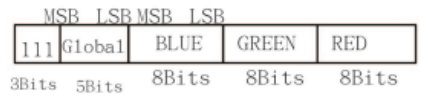
\includegraphics[width=0.6\textwidth]{img/ledpakket.png}
  \caption{Schema van een led-pakket}
  \label{fig:ledpakket}
\end{figure}

\begin{figure}
  \centering
  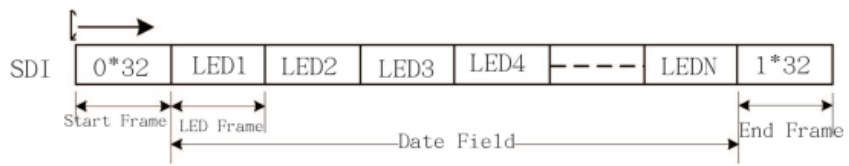
\includegraphics[width=0.8\textwidth]{img/ledcontrol.png}
  \caption{Schema van het aansturen van een ledstrip}
  \label{fig:ledcontrol}
\end{figure}

Er zijn twee mogelijke manieren om meerdere bytes te versturen over SPI,
via een blokkerende §while§-lus en via een interrupt.
Het is echter ook mogelijk om een interrupt te ontvangen wanneer een byte is
verzonden,
om vervolgens een volgende byte te verzenden. Op die manier kan CPU-tijd
uitgespaard worden, maar dit blijkt zeer lastig foutloos te implementeren.
Het spel gebruikt bijgevolg voorlopig nog de \emph{blocking} aanpak.

Het is handig om te weten wat de maximale frequentie is waarmee alle LED's
kunnen aangestuurd worden.
Hiervoor is het belangrijk te weten dat de microcontroller
een werkfrequentie heeft van \SI{16}{\mega\hertz}
en er maximaal 1 bit per 2 klokcycli kan verstuurd worden over SPI.
Er zijn 16 LED's, dit geeft een maximale frequentie van \SI{15625}{\hertz}.
In de praktijk zal deze limiet dus waarschijnlijk nooit een probleem leveren.

Dit systeem wordt aangestuurd door het volgende, het \emph{graphics} systeem.

\subsection{Graphics}
\label{sec:ledtiming}
Het graphics systeem bepaalt alle tijdstippen waarop leds moeten worden aangestuurd samen met welke leds op elk van deze tijdstippen moeten worden aangestuurd.

Zoals op het schema in figuur~\ref{fig:structuur} is te zien, neemt de graphics laag input van de game engine en de hoeksnelheidsmeting component.
Van de game engine krijgt de graphics laag het volgend af te beelden scherm binnen. Dit is een array van sprites waarvan het aantal
elementen gelijk is aan het aantal sprites die op het volgende scherm moeten getoond worden. Indien bijvoorbeeld een zwart scherm
gewenst is, dan wordt een lege array meegegeven. Van de hoeksnelheidsmeting component wordt de meest recente rotatietijd opgevraagd.
Dit is het aantal klokslagen van Timer/Counter1 nodig voor een volledige rotatie van de schijf.

\subsubsection{Vertaling naar queue items}
De graphics laag begint met het vertalen van alle sprites naar queue elementen.
Een sprite is als volgt opgebouwd:
\begin{itemize}
	\item Kleur sprite
	\item Positie
	\begin{itemize}
		\item Hoek (0 tot 3599)
		\item Straal (0 tot 11)
	\end{itemize}
\end{itemize}

Een queue item is als volgt opgebouwd:
\begin{itemize}
	\item Timing (0 tot rotatietijd)
	\item Een array §kleur_en_index[]§
	\begin{itemize}
		\item Kleur en index
			\begin{itemize}
				\item Kleur sprite
				\item Index (0 tot 15)
			\end{itemize}
	\end{itemize}
\end{itemize}

De sprite kleur wordt rechstreeks doorgegeven. Uit de hoek wordt bepaald boven welk segment de sprite valt, of met andere woorden welke 
index van de ledstrip moet worden aangestuurd. Uit de hoek en de straal wordt berekend wanneer de uitsparing op de gekozen straal op de 
gespecifieerde hoek staat. De timing is relatief t.o.v. de rotatiesnelheid en gebruikt als eenheid ook de counter waarden van Timer/Counter1.

Initieel is er een één op één relatie tussen sprites en queue items. Voor elke sprite wordt één queue item aangemaakt, de array ‘kleur 
en index’en bevat dus telkens één element.

Na deze stappen is de queue klaar om de nieuwe globale queue te worden


\subsubsection{Queue van queue items}
Er is steeds een globale queue aanwezig waarop verwerking van queue items wordt gedaan, in het volgende punt volgt hier meer uitleg 
over. Als een nieuw scherm moet worden afgebeeld wordt een nieuwe queue klaargemaakt op de achtergrond, alvorens zijn lancering als 
globale queue.

Een queue ziet er als volgt uit:
\begin{itemize}
	\item Front
	\item Count
	\item Een array §Queue_items[]§
\end{itemize}

Count houdt bij hoeveel queue items aanwezig zijn in de array van queue items. Front houdt de index bij van de volgende queue item die 
die moet verwerkt worden.

Alle queue items worden in een queue geplaatst waarin ze om te beginnen chronologisch gesorteerd worden op timings. Hiervoor is 
sorteeralgoritme geschreven met tijdscomplexiteit \(O\left (\frac{n^2-1}{2} \right )\) of \(O\left (
  n^2 \right )\), voor enkele af te beelden sprites lijkt dit voorlopig voldoende efficiënt. 
Vervolgens wordt de queue door een aggregatiestap geloodst waarin timings die elkaar zeer dicht opvolgen worden samen geplaatst onder 
één queue item, met één timing en meerdere ‘kleur en index’ instanties. Als laatste wordt de front eigenschap ingesteld op basis van de 
huidige TCNT1 waarde, de timing van het queue item op index front moet de eerste zijn die vanaf TCNT1 zal plaatsvinden.

Na deze stappen is de queue klaar om de nieuwe globale queue te worden


\subsubsection{Queue verwerken}
Twee interrupts, werker A en werker B, verwerken de globale queue. Deze interrupts worden getriggerd op een compare match met TCNT1 en 
respectievelijk OCR1A of OCR1B. Merk op dat deze interrupts net zoals de interrupt van de snelheidssensor van Timer/Counter1 afkomstig 
zijn. Dit is handig omdat de snelheidssensor TCNT1 reset bij elke nieuwe toer, en omdat de rotatietijd van de snelheidssensor en de 
timings van de graphics laag niet verschaald zijn tegenover elkaar. De sensor maakt van TCNT1 een tijdsas voor de graphicslaag.

Werker A wordt getriggerd op de timing van het front queue item. De taak van werker A bestaat ten eerste uit alle leds en indexes van 
het front queue item in de led_array die in de hoofdlus naar de leddriver gestuurd wordt te stoppen. Ten tweede stelt werker A de 
volgende timing van werker B in in register OCR1B. Dit is telkens op een vaste offset vanaf OCR1A, in het project is dit 100 
klokslagen.

Werker B wordt 100 klokslagen na werker A getriggerd en zet ten eerste de aangezette leds terug uit. En vervolgens neemt hij de 
volgende timing voor werker A uit de Queue en stopt deze in OCR1A. Na de hoogste timing wordt de laagste timing terug gegeven.


\subsubsection{Ter info}
De rotatietijd is ongeveer \num{13000} slagen wanneer aan 19 toeren per seconde gewerkt wordt.

\subsubsection{Staving}
Er is voor deze aanpak met queues gekozen om de hoge resolutie die mogelijk is met dit scherm uit te buiten. De resolutie in de 
omtrekrichting is met deze aanpak 3600, omdat de hoek component van een sprite een waarde van 0 tot 3599 is. De queue aanpak leent zich 
ook zeer goed voor ons spel omdat we met enkele lichtpunten die heel vlot kunnen bewegen genoeg hebben.

\subsubsection{Kritische noot}
De volledig correcte implementatie van het queue systeem is niet verwezenlijkt bij gebrek aan planning en tijd. De grootste bouwstenen 
zijn wel geïmplementeerd, op de meeste delen van het scherm is de werking correct, al zijn er nog een paar te vermijden zones.

Er zijn al enkele problemen gevonden in de werking van het graphics-systeem. Een
eerste is dat er telkens een nieuwe queue aangemaakt is, deze gekopieerd wordt
naar de globale queue. Dit neemt vrij veel tijd in beslag en zou
verantwoordelijk kunnen zijn voor de te vermijden zones. Er is ook een
functieoproep gevonden waarin deze queue als argument wordt meegegeven, dit zal
nog een kopie genereren. Dit laatste kan opgelost worden door een pointer naar
de queue mee te geven. Ook werd ontdekt dat bepaalde stukken data die in de
queue zitten, eigenlijk uit \emph{scope} gaan voor ze gebruikt worden. Daardoor
is het mogelijk dat de geheugenlocaties overschreven worden met andere data, en
het scherm rare dingen weergeeft.

\subsection{Game engine}
Intern wordt alles dat moet weergegeven worden, voorgesteld door een
\emph{entity}, dit zijn bijvoorbeeld kogels en spelers. Een \emph{entity} bevat
telkens informatie over de positie, in poolcoördinaten, en LED-informatie. De
meeste \emph{entities} bevatten ook extra informatie die intern nodig is, zoals
de levenskracht van een speler.

De game engine werkt op een relatief eenvoudig principe.
Op regelmatige basis wordt de functie §uint8_t tick()§
opgeroepen. Dit gebeurt door continu een functie §maybe_tick()§ op te roepen,
die controleert of een variabele aan staat, en een tick uitvoert indien dit zo
is. Deze \emph{flag} wordt aangezet door een interrupt die 30 keer per seconde
activeert, met behulp van Timer/Counter0 in CTC mode. Met de telwaarde van $255$
en prescaler van $1024$ wordt ongeveer \SI{30}{\hertz} bekomen. Indien mogelijk
kan dit versneld worden. De 8 bits zijn hiervoor meer dan voldoende.

In een \emph{tick} gebeurt het volgende:
\begin{enumerate}
\item \emph{Tick alle entities}, entities hebben een §tick()§ functie,\\
  bijvoorbeeld §player_tick(Player *p)§, die ervoor zorgt dat de entity zich
  verplaatst volgens zijn snelheid en eventueel reageert op invoer.

\item \emph{Controleer voor botsingen}, in deze stap wordt getest of er
  kogels een schip geraakt hebben, en eventueel levens van deze speler worden
  afgenomen.

\item \emph{Check voor het einde van het spel} door te controleren of beide
  spelers nog in leven zijn. Dit bepaalt de returnwaarde van deze functie,
  §true§ wanneer het spel moet verder gaan, anders §false§.
\end{enumerate}

Alle kogels die op een moment in het spel zijn, worden weergegeven in een array
met vaste grootte, momenteel is dit de willekeurig gekozen waarde 20. Wanneer
er dus al 20 kogels in het spel zijn en een speler probeert te schieten, zal er
niks gebeuren. Om te voorkomen
dat kogels te lang blijven rondvliegen, hebben ze een maximale levensduur,
wanneer deze op nul komt, verdwijnt de kogel. Uiteindelijk willen we kogels
langzaam laten donkerder worden wanneer ze deze limiet bereiken. Ze zakken apart
daarvan langzaamaan naar beneden.

\subsubsection{Start- en eindschermen}
De game engine is ook verantwoordelijk voor het tonen van een opstart- en
eindscherm. Het startscherm is een eenvoudig groen scherm dat het
graphicssysteem omzeilt. Waneer beide joysticks omhoog geduwd worden, start het
spel.

Wanneer een speler wint, krijgt het hele scherm de kleur van deze speler. Om te
herstarten, moet de microcontroller herstart worden. De game engine houdt
daarvoor bij in welke fase het spel zich bevindt.

\subsection{Joysticks}
De \emph{game engine} moet weten in welke posities de joysticks staan,
deze zijn relatief eenvoudig om uit te lezen.
Ze bestaan telkens uit vier NO schakelaars, één per richting.
Aangezien elke joystick op een aparte \emph{port} van de microcontroller
aangesloten is, kan met een simpele §NOT§ operatie en enkele bitshifts een
consistente weergave gegenereerd worden, met 1 bit per richting die hoog is
wanneer de schakelaar actief is. Hiertoe moeten ook de pullups geactiveerd
worden. De driver voor de joysticks controleert ook welke schakelaars sinds de
laatste tick actief zijn geworden, en slaat deze apart op.

Enkele gemaksfuncties werden toegevoegd om uit deze bitweergave te bepalen of
een gekozen richting actief is.

\subsection{Fysieke constructie}
De fysieke constructie is een rechtstaand licht hellend display met voldoende
ruimte voor de elektronica en bedrading. De gehele constructie werd ontworpen
in het CAD-pakket Siemens NX 11 en voornamelijk uitgesneden op een lasercutter,
op een paar uitzonderingen na.

De draaischijf is op de lasercutter gemaakt en bestaat uit \SI{2}{\milli\meter} dikke zwarte ABS.
De schijf bevat 13 gaatjes, goed voor een straalresolutie van 13 pixels. De pixels
zijn gerangschikt in twee spiralen opdat buren veraf van elkaar zouden liggen. Zo
wordt de lichtvervuiling in een aangrenzend segmenten minimaal benadrukt door
zover mogelijk verwijderd te zijn van een sprite.

De segmenten zijn met een breekmes op een snijplank gemaakt uit een wit PVC vel.
Er zijn 16 segmenten en elk segment heeft één led die gemonteerd is op een wand
van de behuizing grenzend aan de cirkel. Het wit plastic zorgt voor een goede
diffusie van het licht van de ledjes.

Dat het aantal segmenten en gaten niet gelijk is aan elkaar komt doordat geen
twee gaten zich tegelijkertijd in hetzelfde segment mogen bevinden. Waarom bij
16 segmenten voor 13 gaten gekozen is wordt duidelijk gemaakt in figuur~\ref{fig:duiding1316}. De
rood aangeduide stukjes staan ter hoogte van het binnenste gaatje en zijn even
lang, de oranje lijnen zijn tonen de segmenten.

\begin{figure}
  \centering
  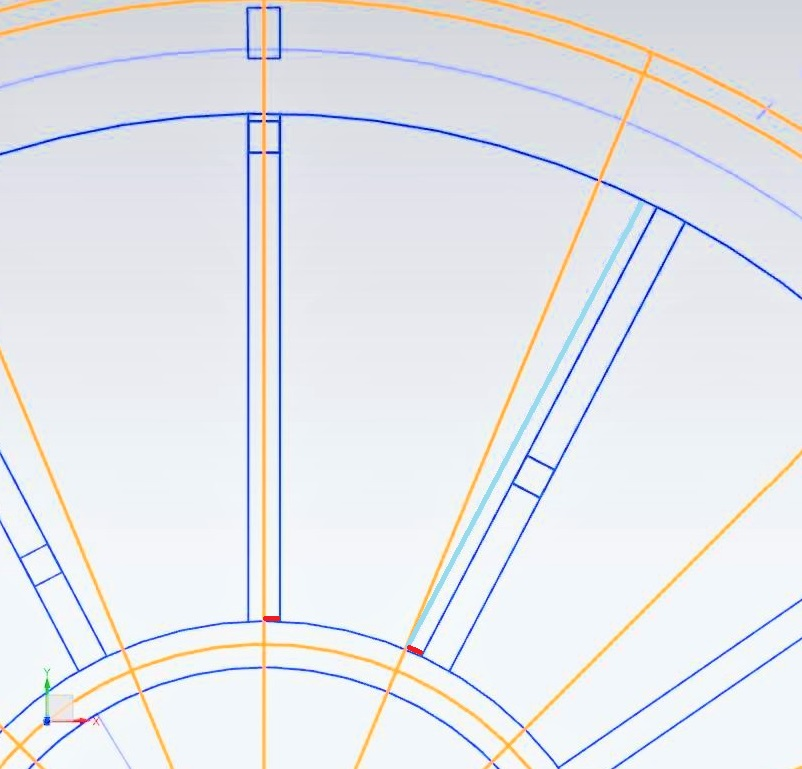
\includegraphics[width=0.6\textwidth]{img/16vs13.jpg}
  \caption{Duiding 16 segmenten 13 gaten}
  \label{fig:duiding1316}
\end{figure}

De sensorhouder is een klein ge-3D-print stuk dat de sensor op zijn plaats
houdt. Dit is zichtbaar in figuur~\ref{fig:sensorhouder}.

De behuizing is gemaakt uit \SI{3}{\milli\metre} dik MDF plaatmateriaal en is volledig demonteerbaar.
Op de behuizing kan een scherm uit een \SI{3}{\milli\metre} dikke plexiplaat geplaats worden. De plaat is te zien in figuur~\ref{fig:plexiplaat}.

\begin{figure}
  \centering
  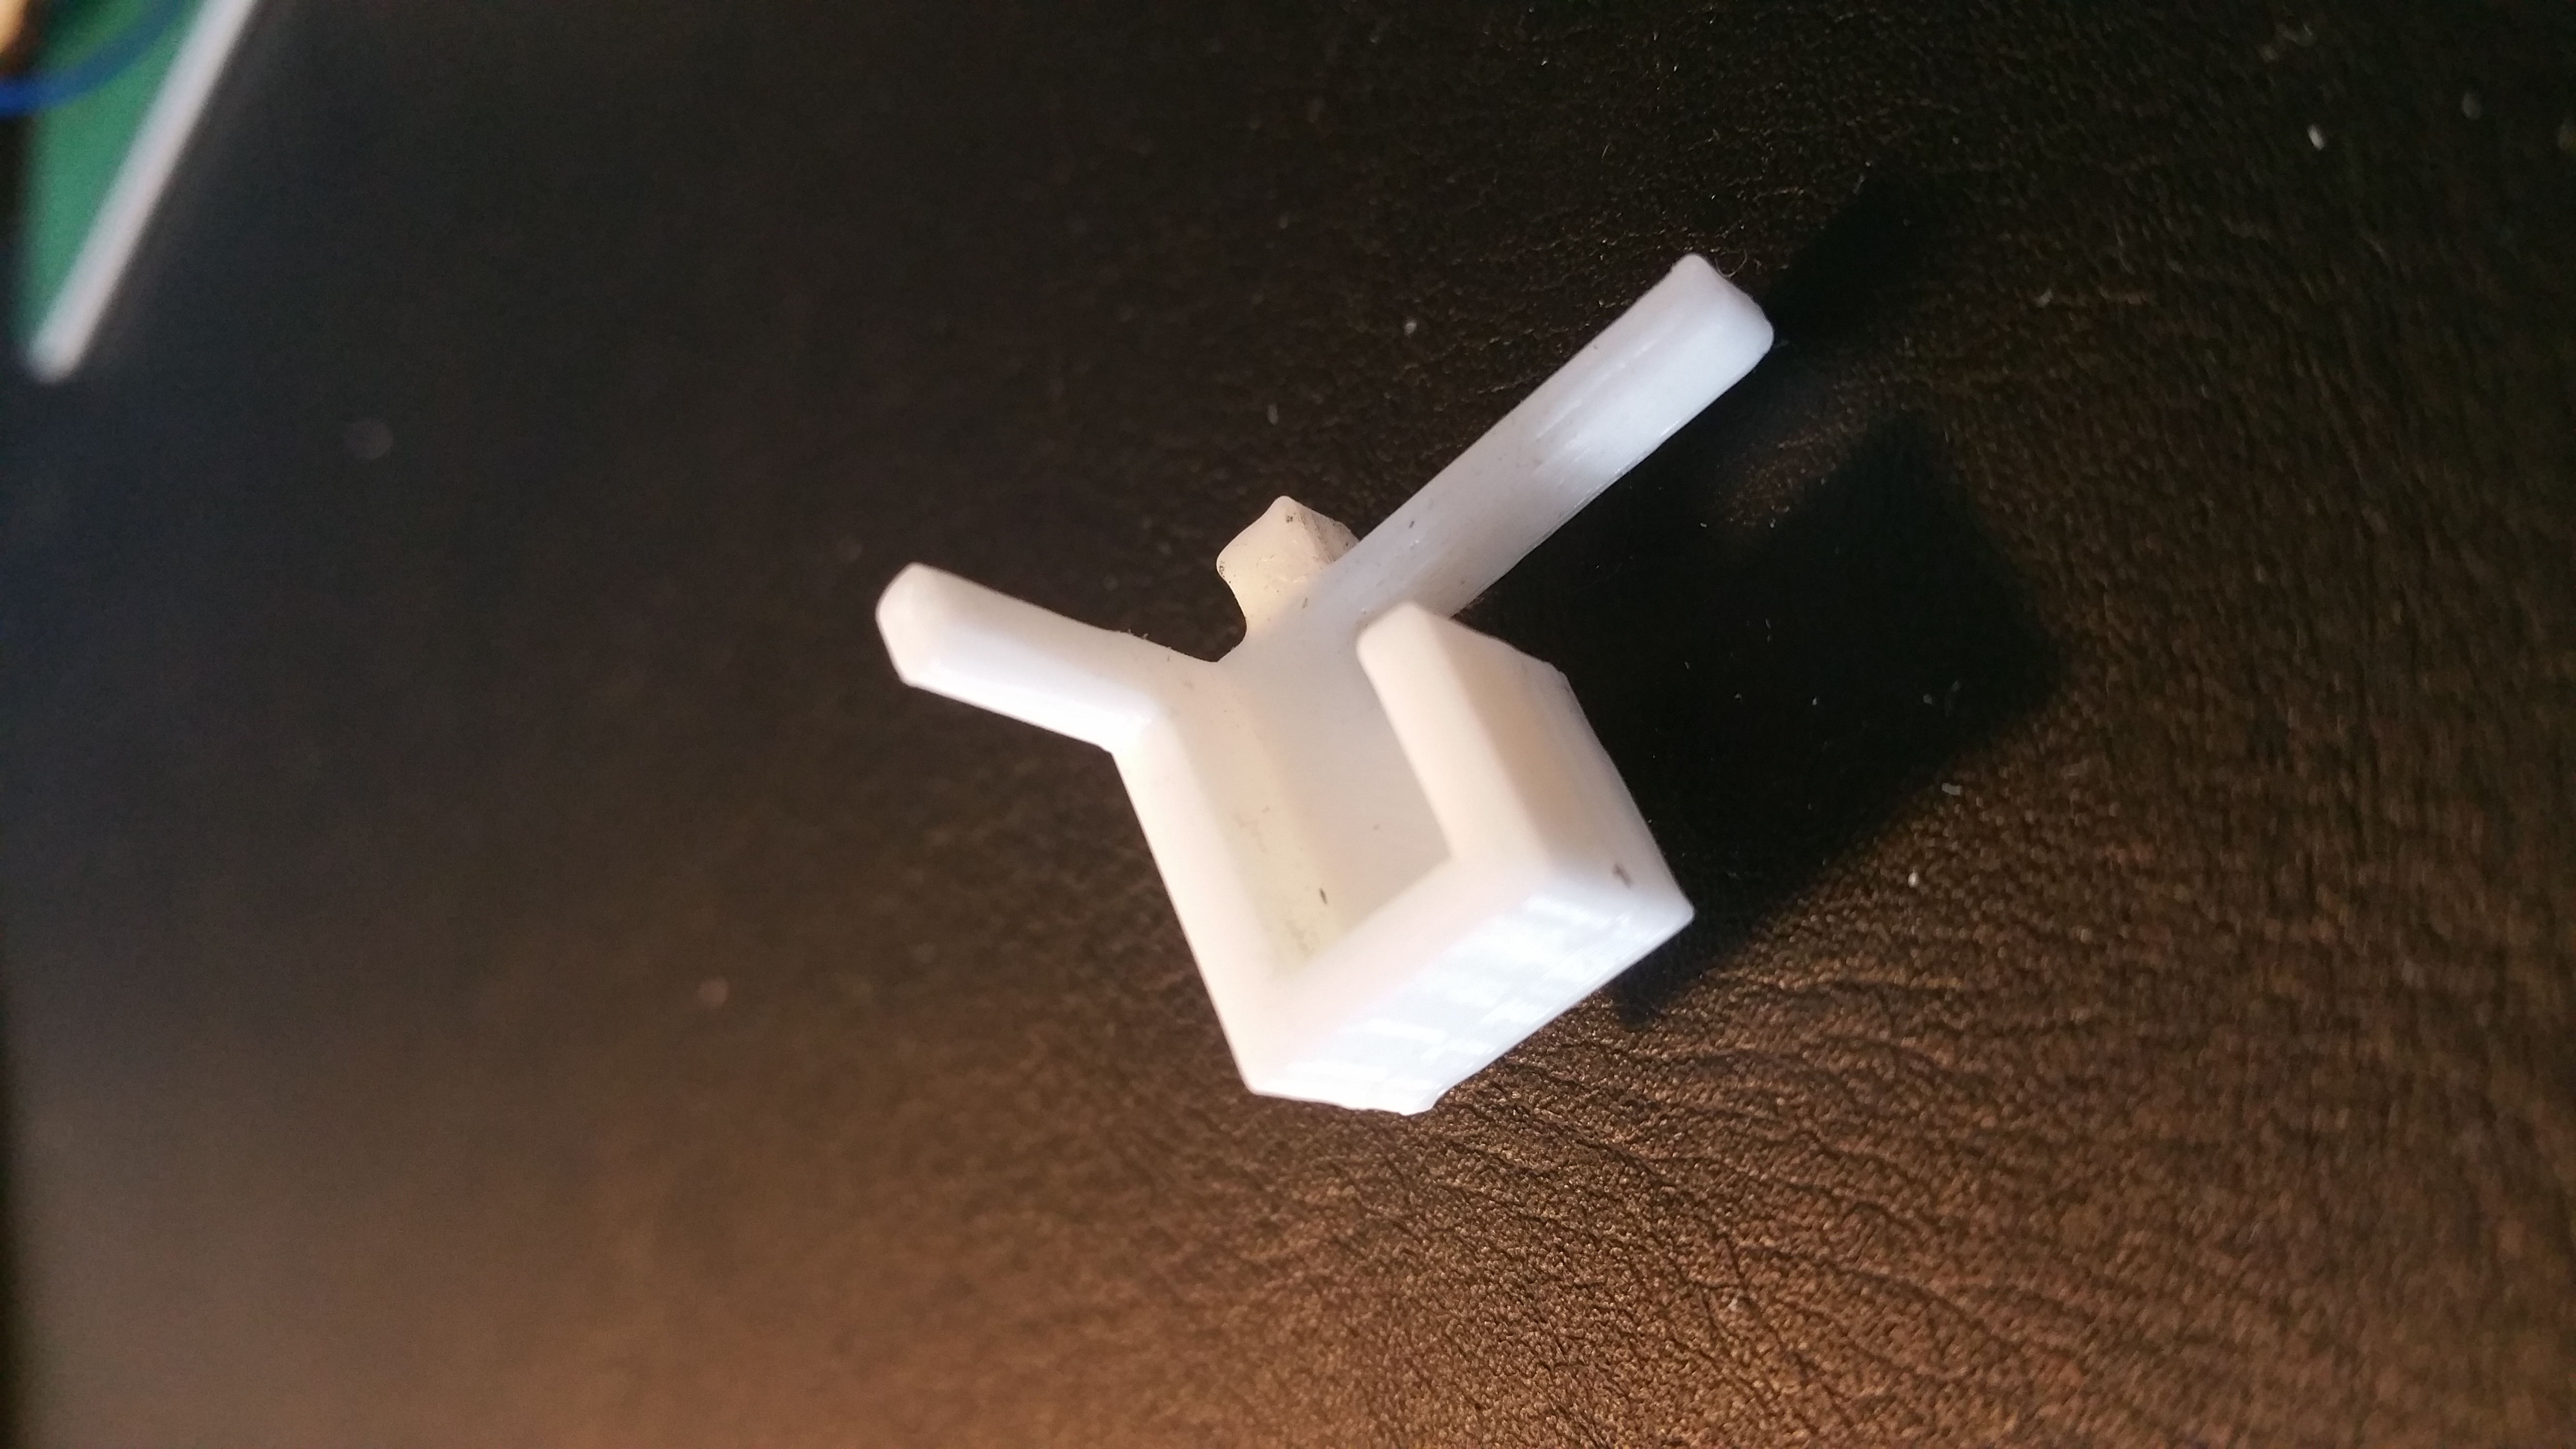
\includegraphics[width=0.6\textwidth]{img/SensorHouder.jpg}
  \caption{Ge-3D-printe sensorhouder}
  \label{fig:sensorhouder}
\end{figure}

\begin{figure}
  \centering
  \includegraphics[width=0.6\textwidth]{img/PlexiPlaat.jpg}
  \caption{Plexi scherm}
  \label{fig:plexiplaat}
\end{figure}

\section{Openstaande Problemen}
Er is nog wat werk aan de fysieke constructie van de schijf en we twijfelen nog
over het aantal sectoren. Het beeld wordt heel instabiel van zodra de game
engine wordt verbonden, er werd dus besloten om een animatie te demonstreren in
plaats van het spel, bij gebrek aan tijd om deze problemen op te lossen.
Bij gevolg is de grote hoeveelheid code in de engine ongebruikt.

Verder zijn er nog enkele verbeteringen te maken in de \emph{game engine},
zo kan het spel niet herstart worden zonder de microcontroller te resetten.

\section{Taakverdeling en Samenwerking}
De motordriver werd geschreven door Marieke. Zij schreef ook de code die voor de
juiste timing zorgt en de optische sensor uitleest en ontwierp en bouwde de
behuizingen. Na de aanpassing van de schijf, herschreef zij het \emph{graphics}-systeem.

De game engine werd gedaan door Stef,
net zoals uitlezen van joysticks en debugfunctionaliteit.

De structuur en layout van het verslag is door Stef, de inhoud werd verdeeld
naar specialiteit.

Onze samenwerking gebeurt via Git en
GitHub\footnote{\url{https://github.com/Epse/MCU_Project_PlanetFight}}. Taken worden
verdeeld via \emph{issues} op GitHub. Iedereen werkt aan een apart deel van de
code of de hardware, die regelmatig samen worden gezet.

\section{Conclusie en Toekomstig Werk}
Voor de specificatie van het project, zie tabel~\ref{tbl:specs}.
Dit project is bijzonder ambitieus, zeker voor een team bestaande uit twee
personen.

Het had leuk geweest moest het oorspronkelijke idee van een schok bij verliezen
geïmplementeerd geraakt zijn, maar hiervoor was geen tijd. Kogels zouden ook wat
vloeiender kunnen verdwijnen. Voor extra moeilijkheid zouden de spelers rond  de
``aarde'' kunnen draaien.

\begin{table}
  \centering
  \begin{tabular}{l|c}
    \hline
    Parameter & Waarde\\
    \hline
    Ingangsspanning Microcontroller & \SI{5}{\volt}\\
    Ingangsspanning ESC & \SI{12}{\volt}\\
    Aantal spelers & 2\\
    Bediening & 2 Joysticks, 4 schakelaars elk\\
    Minimale updatefrequentie & \SI{24}{\hertz}\\
    Weergave & 15 LED's\\
    Radiale resolutie & 13\\
    Omtrekresolutie & 1024\\
    \hline
  \end{tabular}
  \caption{Specificaties}
  \label{tbl:specs}
\end{table}

\end{document}
